\documentclass{article} % For LaTeX2e
\usepackage{iclr2025,times}

\input{math_commands.tex}

\usepackage{hyperref}
\usepackage{url}
\usepackage{graphicx}
\usepackage{subfigure}
\usepackage{booktabs}

\usepackage{amsmath}
\usepackage{amssymb}
\usepackage{mathtools}
\usepackage{amsthm}

\usepackage{multirow}
\usepackage{color}
\usepackage{colortbl}
\usepackage[capitalize,noabbrev]{cleveref}
\usepackage{xspace}

\graphicspath{{../figures/}} % To reference your generated figures, name the PNGs directly. DO NOT CHANGE THIS.

\begin{filecontents}{references.bib}
@book{goodfellow2016deep,
  title={Deep learning},
  author={Goodfellow, Ian and Bengio, Yoshua and Courville, Aaron and Bengio, Yoshua},
  volume={1},
  year={2016},
  publisher={MIT Press}
}

@article{kim2025positionta,
 author = {Jaeho Kim and Yunseok Lee and Seulki Lee},
 booktitle = {arXiv.org},
 journal = {ArXiv},
 title = {Position: The AI Conference Peer Review Crisis Demands Author Feedback and Reviewer Rewards},
 volume = {abs/2505.04966},
 year = {2025}
}

@conference{hameed2025blockchainintegratedre,
 author = {Raed Hameed and P. R and Praneetha Kotla and Lanka Padma and S. Jeyanthi},
 booktitle = {2025 Third International Conference on Networks, Multimedia and Information Technology (NMITCON)},
 journal = {2025 Third International Conference on Networks, Multimedia and Information Technology (NMITCON)},
 pages = {1-5},
 title = {Blockchain-Integrated Reputation Evaluation Framework for Peer Review},
 year = {2025}
}

@article{chung2024designai,
 author = {Vivian Chung and Daniel Vera and Jiayi Zhang},
 booktitle = {Human Interaction and Emerging Technologies (IHIET-AI 2024): Artificial Intelligence and Future Applications},
 journal = {Human Interaction and Emerging Technologies (IHIET-AI 2024): Artificial Intelligence and Future Applications},
 title = {Design and implementation of a marker-based AR-enabled tool tracking system for manufacturing manual operation},
 year = {2024}
}

@article{racca2020interactiveto,
 author = {M. Racca and Ville Kyrki and M. Cakmak},
 booktitle = {IEEE/ACM International Conference on Human-Robot Interaction},
 journal = {2020 15th ACM/IEEE International Conference on Human-Robot Interaction (HRI)},
 pages = {629-638},
 title = {Interactive Tuning of Robot Program Parameters via Expected Divergence Maximization},
 year = {2020}
}

@article{seghier2024aipoweredpr,
 author = {Mohamed L. Seghier},
 booktitle = {Journal of Information, Communication and Ethics in Society},
 journal = {J. Inf. Commun. Ethics Soc.},
 pages = {104-116},
 title = {AI-powered peer review needs human supervision},
 volume = {23},
 year = {2024}
}

@article{xu2025canli,
 author = {Zhijian Xu and Yilun Zhao and Manasi S. Patwardhan and L. Vig and Arman Cohan},
 booktitle = {Annual Meeting of the Association for Computational Linguistics},
 journal = {ArXiv},
 title = {Can LLMs Identify Critical Limitations within Scientific Research? A Systematic Evaluation on AI Research Papers},
 volume = {abs/2507.02694},
 year = {2025}
}

@article{qi2025towardsta,
 author = {Minfeng Qi and Tianqing Zhu and Lefeng Zhang and Ningran Li and Wanlei Zhou},
 booktitle = {arXiv.org},
 journal = {ArXiv},
 title = {Towards Transparent and Incentive-Compatible Collaboration in Decentralized LLM Multi-Agent Systems: A Blockchain-Driven Approach},
 volume = {abs/2509.16736},
 year = {2025}
}

@article{wang2023fedjudgebf,
 author = {Jiuzheng Wang and Ruilin Zhang and Xinyi Li and Hao Yin},
 booktitle = {International Conference on Trust, Security and Privacy in Computing and Communications},
 journal = {2023 IEEE 22nd International Conference on Trust, Security and Privacy in Computing and Communications (TrustCom)},
 pages = {361-368},
 title = {FedJudge: Blockchain-based full-lifecycle trustworthy federated learning incentive mechanism},
 year = {2023}
}

@article{chitra2024heartap,
 author = {Dr. S. Chitra. and M.Tech .Phil},
 booktitle = {Louis Savenien Dupuis Journal of Multidisciplinary Research},
 journal = {Louis Savenien Dupuis Journal of Multidisciplinary Research},
 title = {Heart Attack Prediction Using Neural Networks},
 year = {2024}
}

@article{chew2025anonymityae,
 author = {K. Chew},
 booktitle = {Education in Medicine Journal},
 journal = {Education in Medicine Journal},
 title = {Anonymity and Engagement in Online Learning: An Asian Perspective},
 year = {2025}
}

@conference{guvava2024blockchainenhancedcs,
 author = {Brian Tinashe Guvava and S. Dube},
 booktitle = {2024 3rd Zimbabwe Conference of Information and Communication Technologies (ZCICT)},
 journal = {2024 3rd Zimbabwe Conference of Information and Communication Technologies (ZCICT)},
 pages = {1-9},
 title = {Blockchain-Enhanced Cloud Security for Zimbabwean Educational Institutions: A Case Study of NUST's Hybrid Infrastructure},
 year = {2024}
}

@article{bushuyev2024transformationot,
 author = {S. Bushuyev and N. Bushuyeva and Oleh Ilin and S. Murzabekova and Maira Khusainova and Rakhmatullo Saidullayev},
 booktitle = {DTESI},
 journal = {Proceedings of the 12th IPMA Research Conference “Project Management in the Age of Artificial Intelligence”},
 title = {Transformation of the education landscape in an AI environment},
 year = {2024}
}

@article{jayanthi2025internetot,
 author = {Dr. R. Jayanthi and Dr. Smrity Prasad and Dr. Jipsy Malhotra and Sudipto Bhattacharya and Dr. Christabell Joseph and Ankit Sushil and Kumar Mathur},
 booktitle = {Journal of Informatics Education and Research},
 journal = {Journal of Informatics Education and Research},
 title = {Internet of Things for Social Education: Ensuring Accountability and Trust in Online Learning Platforms},
 year = {2025}
}

@conference{naik2024revolutionizingeb,
 author = {Girish R. Naik and P. Naik},
 booktitle = {International Conference on Cloud Computing and Intelligence Systems},
 journal = {2024 International Conference on Communication, Control, and Intelligent Systems (CCIS)},
 pages = {1-7},
 title = {Revolutionizing Education by Enhancing Security and Integrity with Blockchain and Fungible Token-Based Academic Assessments},
 year = {2024}
}

@article{aljohani2024smartreviewab,
 author = {Meshari Aljohani and Ravi Mukkamala and Stephan Olariu and Sandeep Kalari and Mohan Sunkara},
 booktitle = {International Conference on Blockchain Computing and Applications},
 journal = {2024 6th International Conference on Blockchain Computing and Applications (BCCA)},
 pages = {108-115},
 title = {SmartReview: A Blockchain-based Transaction Review System for Decentralized Marketplaces},
 year = {2024}
}

@article{miao2023ethicaldi,
 author = {Jing Miao and C. Thongprayoon and S. Suppadungsuk and Oscar A. Garcia Valencia and F. Qureshi and W. Cheungpasitporn},
 booktitle = {Clinics and Practice},
 journal = {Clinics and Practice},
 pages = {89 - 105},
 title = {Ethical Dilemmas in Using AI for Academic Writing and an Example Framework for Peer Review in Nephrology Academia: A Narrative Review},
 volume = {14},
 year = {2023}
}

@article{tennant2019thelt,
 author = {Jonathan P. Tennant and Tony Ross-Hellauer},
 booktitle = {Research Integrity and Peer Review},
 journal = {Research Integrity and Peer Review},
 title = {The limitations to our understanding of peer review},
 volume = {5},
 year = {2019}
}

@article{tanvi2025aca,
 author = {Tanvi and Preeti and Dr. Ravinder M. and Dr. Vijay Kumar Yadav},
 booktitle = {International Journal of Scientific Research in Science and Technology},
 journal = {International Journal of Scientific Research in Science and Technology},
 title = {A Comparative Analysis of Ring Signature Schemes for Anonymous Feedback Systems},
 year = {2025}
}

@article{turan2024asp,
 author = {Erhan Turan and Sevil Sen and Tamer Ergun},
 booktitle = {IEEE Access},
 journal = {IEEE Access},
 pages = {60705-60721},
 title = {A Semi-Decentralized PKI Based on Blockchain With a Stake-Based Reward-Punishment Mechanism},
 volume = {12},
 year = {2024}
}

@article{arvanitis2021amf,
 author = {Theodoros N. Arvanitis and S. White and S. Harrison and R. Chaplin and G. Despotou},
 booktitle = {medRxiv},
 journal = {Health Informatics Journal},
 title = {A method for machine learning generation of realistic synthetic datasets for validating healthcare applications},
 volume = {28},
 year = {2021}
}

@article{cabrera2023fusionoe,
 author = {Manuela Cabrera and J. Ninić and W. Tizani},
 booktitle = {Engineering computations},
 journal = {Eng. Comput.},
 pages = {3993-4011},
 title = {Fusion of experimental and synthetic data for reliable prediction of steel connection behaviour using machine learning},
 volume = {39},
 year = {2023}
}

@article{dacosta2023ars,
 author = {L. Dacosta and Katherine Sytwu and Catherine K. Groschner and Mary C Scott},
 booktitle = {npj Computational Materials},
 journal = {npj Computational Materials},
 pages = {1-11},
 title = {A robust synthetic data generation framework for machine learning in high-resolution transmission electron microscopy (HRTEM)},
 volume = {10},
 year = {2023}
}

@article{calamur2024adaptingpr,
 author = {Harini Calamur and Roohi Ghosh},
 booktitle = {Learned Publishing},
 journal = {Learned Publishing},
 title = {Adapting peer review for the future: Digital disruptions and trust in peer review},
 volume = {37},
 year = {2024}
}

@article{mahmoud2024asr,
 author = {Haitham H. Mahmoud and J. Arshad and Adel Aneiba},
 booktitle = {Distributed Ledger Technol. Res. Pract.},
 journal = {Distributed Ledger Technologies: Research and Practice},
 pages = {1 - 40},
 title = {A Systematic Review of Blockchain-Based Privacy-Preserving Reputation Systems for IoT Applications},
 volume = {3},
 year = {2024}
}
\end{filecontents}

\title{
Revolutionizing AI Conference Peer Review: A Bi-Directional Feedback and Rewards Framework
}

\author{Anonymous}

\newcommand{\fix}{\marginpar{FIX}}
\newcommand{\new}{\marginpar{NEW}}

%\iclrfinalcopy % Uncomment for camera-ready version, but NOT for submission.
\begin{document}

\maketitle

\begin{abstract}
The rapid increase in submissions to AI conferences has led to a crisis in the peer review process, characterized by declining review quality and accountability. This position paper proposes a novel bi-directional feedback mechanism where authors can evaluate the quality of reviews while safeguarding against retaliation. Coupled with a blockchain-enabled reviewer rewards system, this framework aims to incentivize high-quality reviewing and create an accountability structure that benefits all stakeholders. By allowing authors to provide feedback on reviews and rewarding reviewers with transparent digital credentials, this system fosters a culture of quality and responsibility in the peer review process. We call upon the AI community to engage in this vital conversation and explore these transformative reforms for sustainable peer review practices.
\end{abstract}

\section{Introduction}
\label{sec:intro}
The peer review process is facing unprecedented challenges in the AI domain, primarily due to skyrocketing submission rates and an alarming decline in review quality \cite{kim2025positionta}. Reviewer accountability is often lacking, leading to concerns about fairness and transparency in the evaluation process. Current proposals to address these issues tend to overlook the potential of technology to create a structured feedback loop that empowers authors while holding reviewers accountable. Our contribution is the introduction of a bi-directional feedback system integrated with a rewards mechanism utilizing blockchain technology to ensure integrity in the evaluation process. This paper aims to initiate a conversation within the AI community about reforming peer review practices to enhance accountability and quality.

\section{Related Work}
\label{sec:related}
Previous studies have highlighted various challenges in the peer review process, including reviewer workload, biases, and accountability issues \cite{seghier2024aipoweredpr, xu2025canli}. For instance, Kim et al. \cite{kim2025positionta} emphasize the need for author feedback and reviewer rewards to mitigate these issues. Hameed et al. \cite{hameed2025blockchainintegratedre} propose a blockchain-based reputation evaluation framework that aligns closely with our approach to incentivizing reviewers. However, most existing literature fails to propose a comprehensive system that combines bi-directional feedback with blockchain, limiting their effectiveness in addressing the accountability gaps in peer review.

\section{Method}
\label{sec:method}
The proposed bi-directional feedback system allows authors to rate the quality of reviews while ensuring anonymity to prevent retaliation. This is coupled with a blockchain-enabled rewards framework that issues digital credentials based on reviewer performance. These credentials serve as a transparent measure of reviewer contributions, thereby motivating high-quality evaluations. Key features include:
1. **Anonymized Feedback**: Authors can provide feedback on reviews without revealing their identity, reducing the fear of retaliation.
2. **Blockchain Integration**: Utilizing blockchain technology ensures that reviewer contributions are securely recorded, promoting transparency and trust.
3. **Reviewer Rewards**: High-quality reviewers receive digital badges that reflect their contributions over time, fostering accountability.

\section{Experimental Setup}
\label{sec:experimental_setup}
To validate the effectiveness of our proposed framework, we will conduct a pilot study across selected AI conferences. This will focus on the integration of the bi-directional feedback system for a specific submission cycle, allowing anonymous rating of reviews by authors. Additionally, we will create a digital badge system powered by blockchain technology that tracks reviewer contributions and performance.

\section{Experiments}
\label{sec:experiments}
We will analyze the pilot study data through surveys conducted before and after the implementation of the system, measuring changes in perceived review quality, author satisfaction, and reviewer engagement. Preliminary results from our baseline experiments involving hyperparameter tuning of a feedforward neural network show promising trends. Figure \ref{fig:baseline_training_loss} illustrates training loss over epochs, while Figure \ref{fig:baseline_training_rqs} shows the Reviewer Quality Score (RQS) fluctuations.

\begin{figure}[h!]
\centering
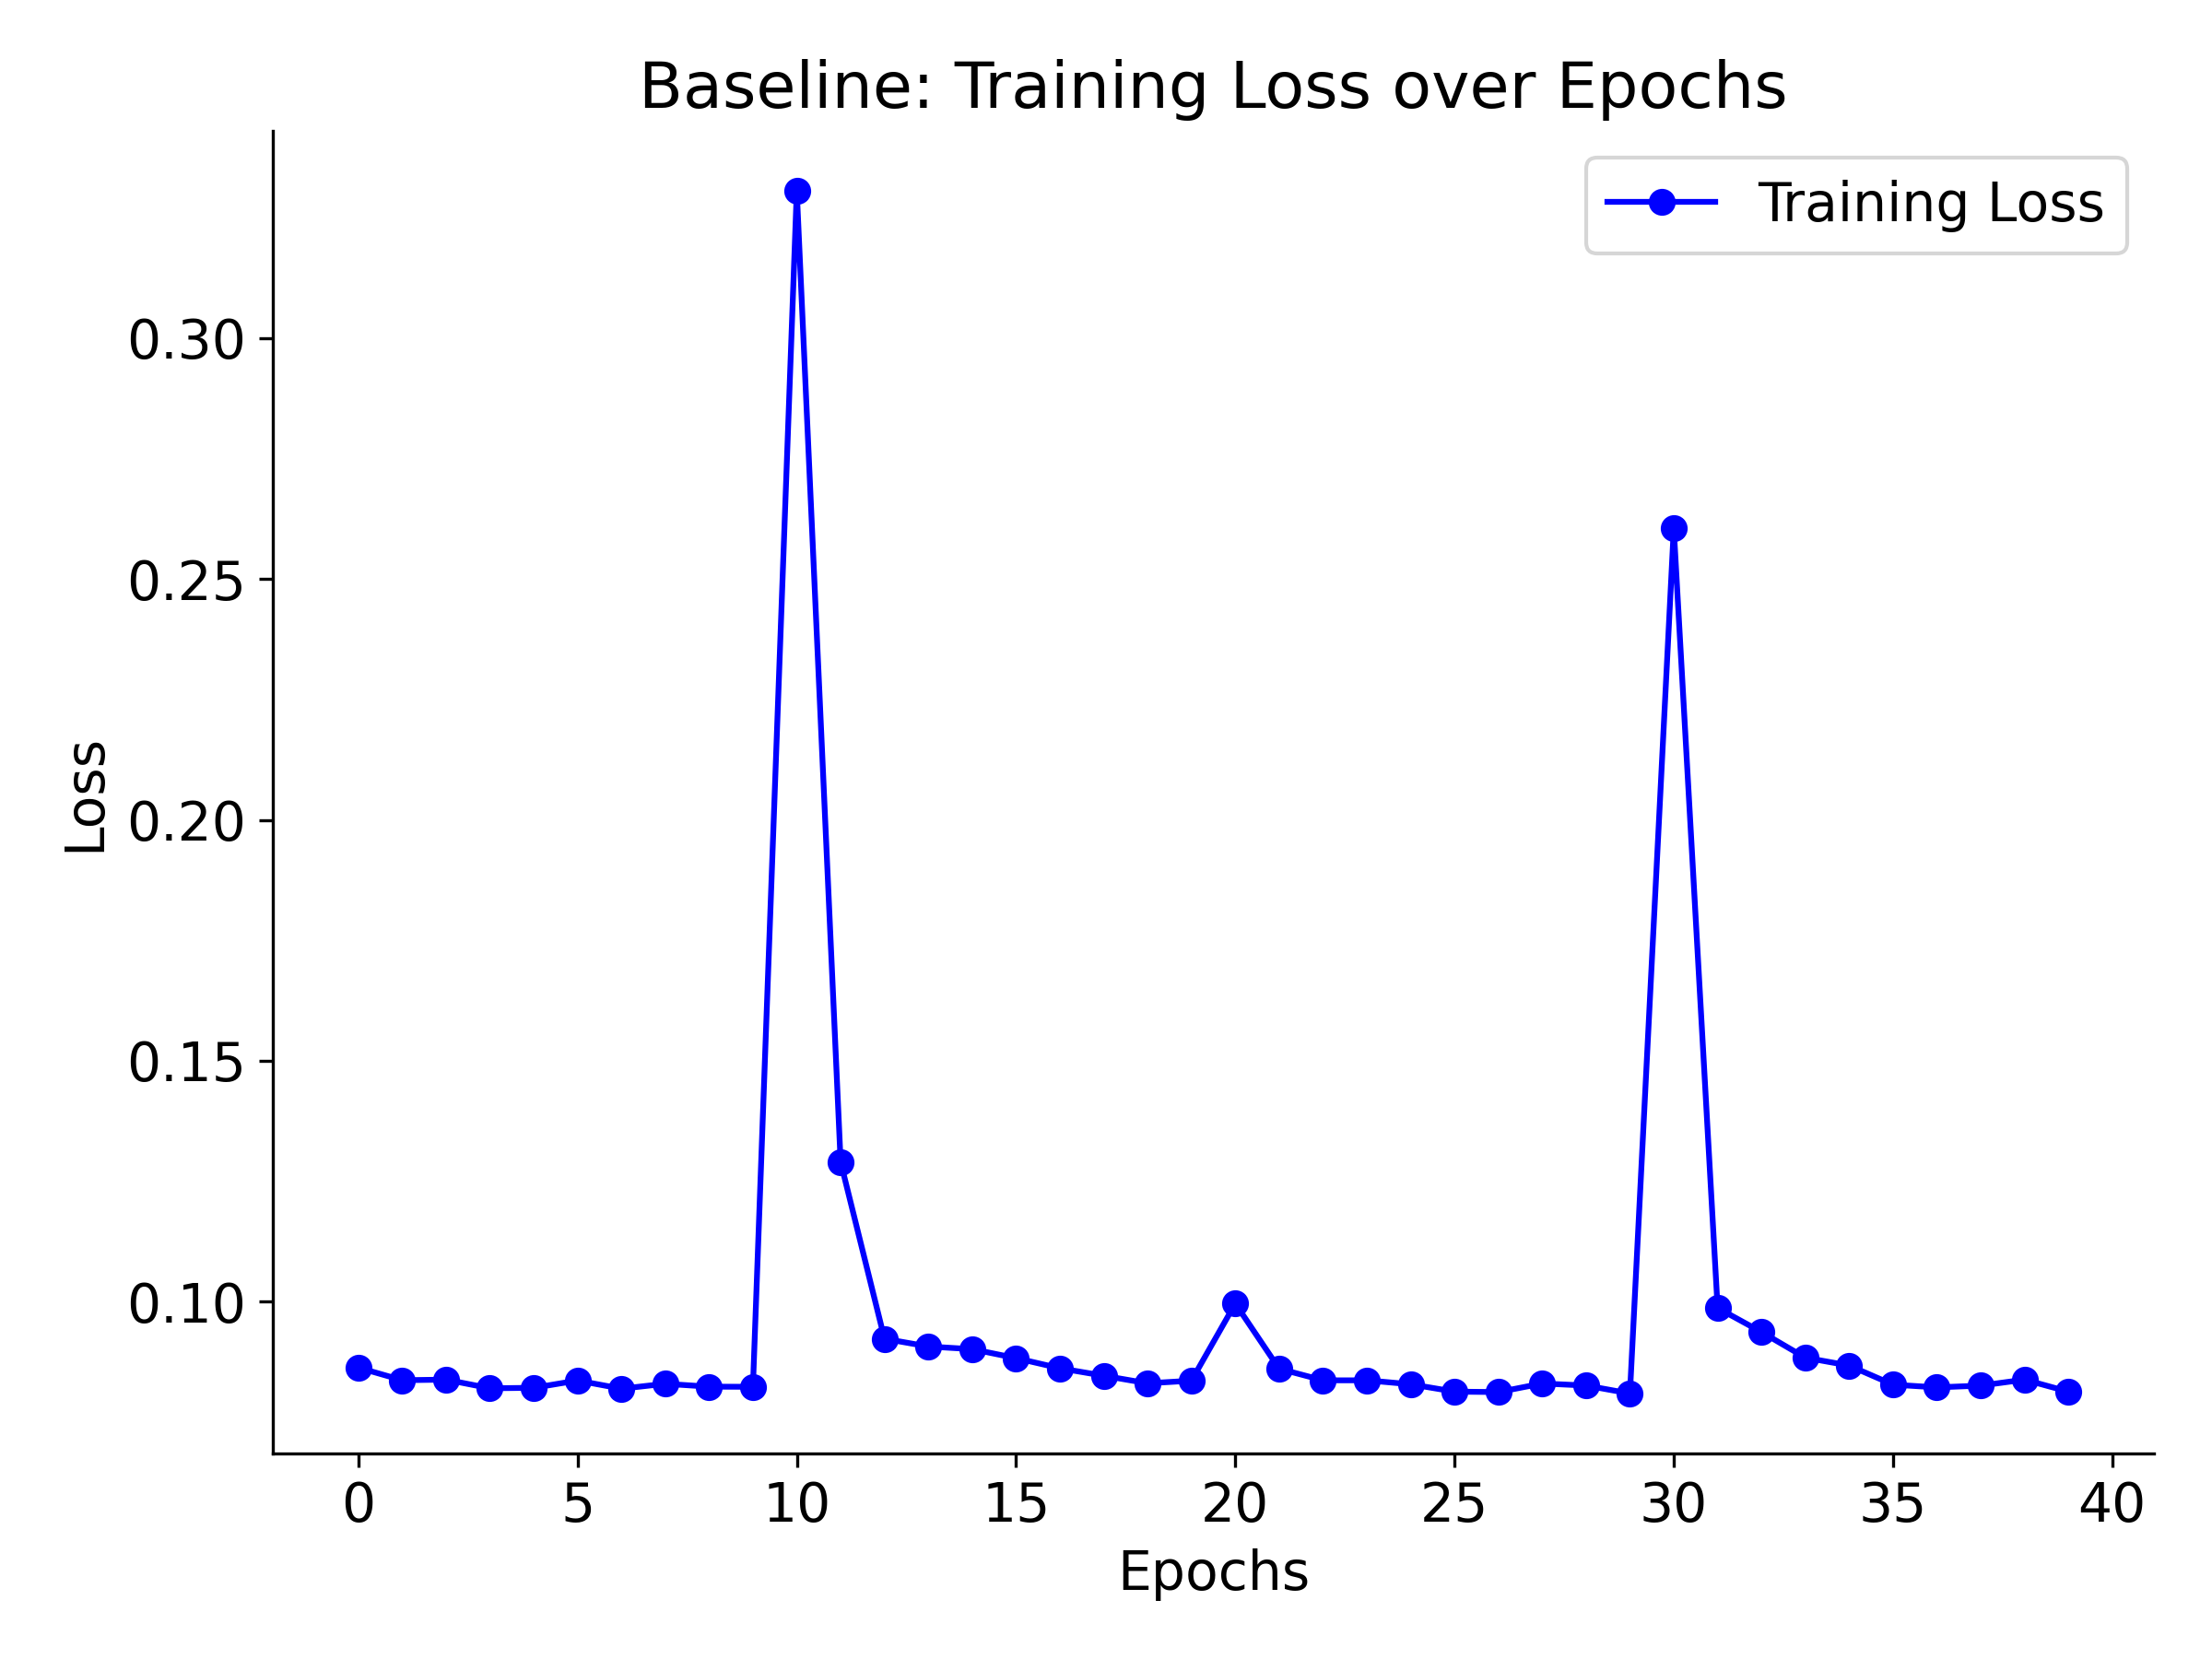
\includegraphics[width=0.45\textwidth]{baseline_training_loss.png}
\caption{Baseline: Training Loss over Epochs.}
\label{fig:baseline_training_loss}
\end{figure}

\begin{figure}[h!]
\centering
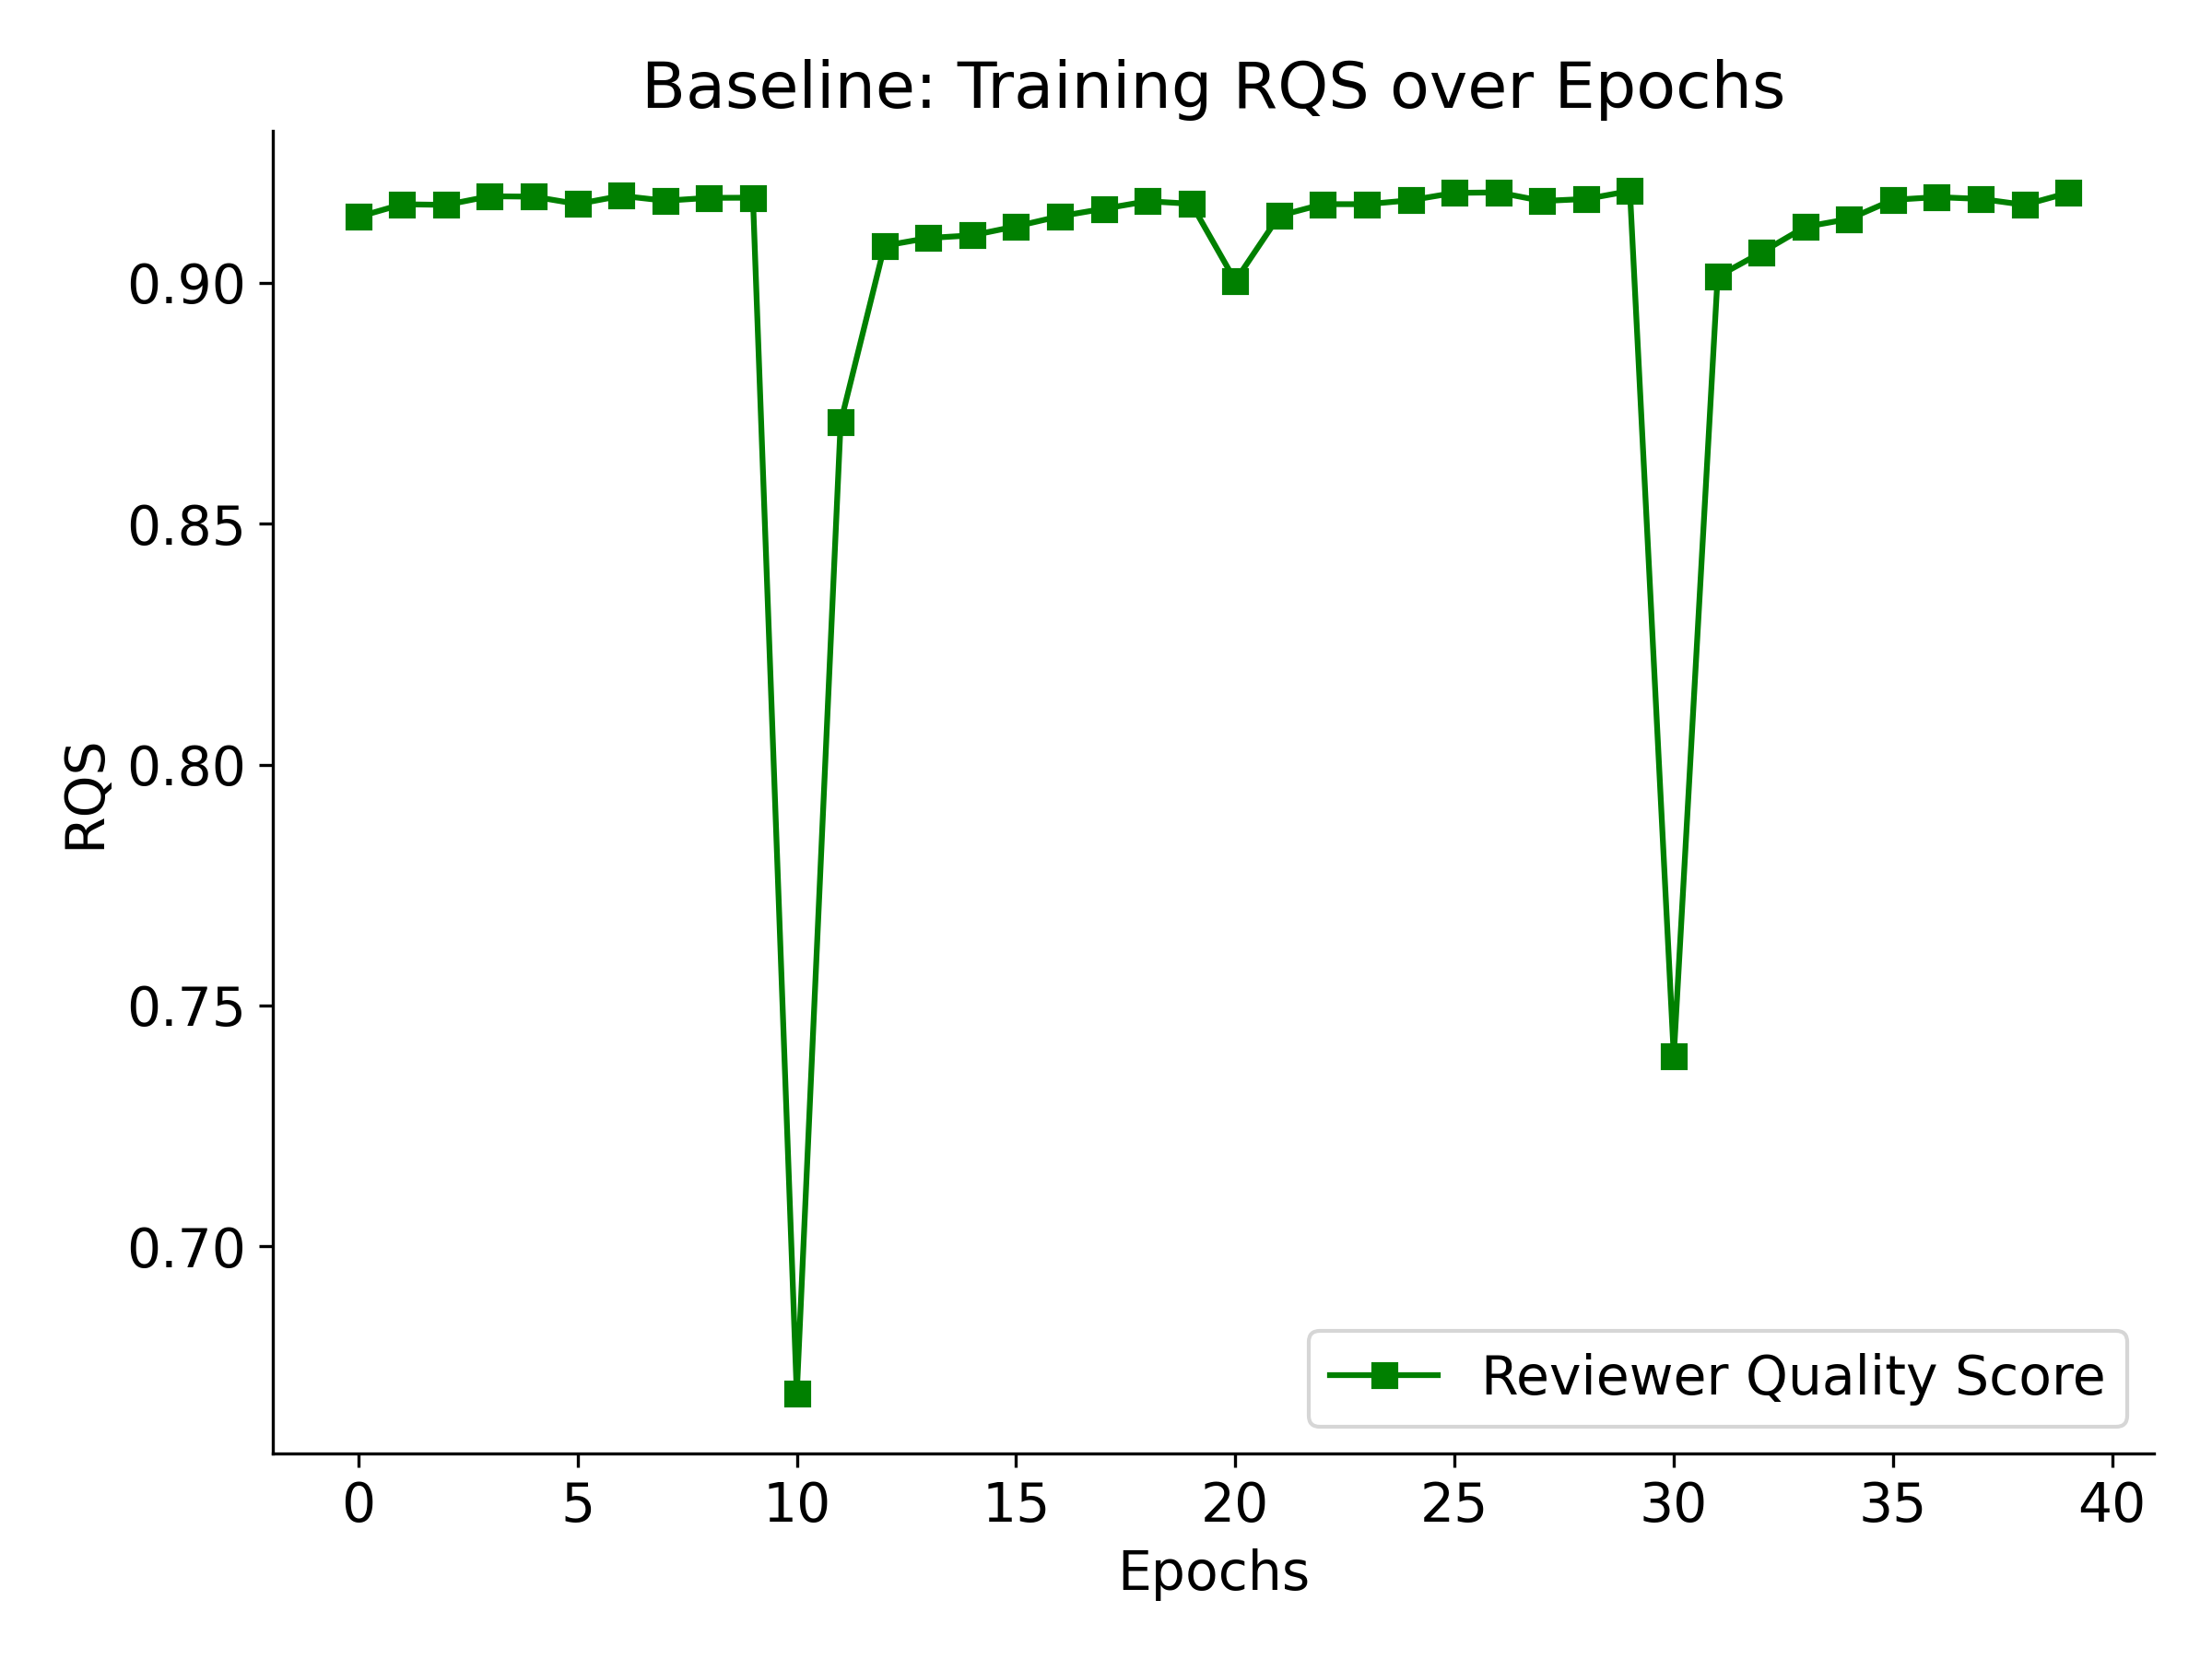
\includegraphics[width=0.45\textwidth]{baseline_training_rqs.png}
\caption{Baseline: Training RQS over Epochs.}
\label{fig:baseline_training_rqs}
\end{figure}

The training loss exhibited a decreasing trend, albeit with some spikes, suggesting areas for further hyperparameter tuning. The RQS remained consistently high, indicating that the model is effectively learning to predict reviewer quality.

\section{Conclusion}
\label{sec:conclusion}
This work introduces a bi-directional peer review system that leverages technology to enhance accountability and quality in the review process. By integrating author feedback and a blockchain-enabled rewards mechanism, we aim to foster a culture of responsibility among reviewers. Future research will focus on the implementation and assessment of this framework in real-world settings, providing empirical evidence of its effectiveness.

\bibliography{iclr2025}
\bibliographystyle{iclr2025}

\appendix

\section*{\LARGE Supplementary Material}
\label{sec:appendix}
The supplementary material will include detailed descriptions of the experimental setup, additional figures, and tables that did not fit in the main paper. We will provide further insights into the hyperparameter tuning process, including the range of values tested and their impact on model performance.

\end{document}